\section{État actuel du projet et prévision pour la prochaine soutenance}
        
        Voici un tableau d'avancement des tâches réalisé et de nos prévisions pour la dernière soutenance : \\ \\
    
        {\normalsize
    	\begin{tabular}{|p{7cm}|p{2.4cm}|p{2.4cm}|}
    		\hline
    		Tâches & Actuellement & Objectif final \\
    		\hline
    		Système de fichier & 100\% & 100\% \\
    		\hline
    		Sauvegarde & 100\% & 100\% \\
    		\hline
    		Compression & 50\% & 100\% \\
    		\hline
    		Chiffrement & 95\% & 100\% \\
    		\hline
    		Site web & 100\% & 100\% \\
    		\hline
    		Interface graphique & 75\% & 100\% \\
    		\hline
    	\end{tabular}
    	\label{répartition}}

\newpage

\section{Sauvegarde}
    
    \subsection{Système de fichier}
        \subsubsection{Rappel de la soutenance 1:}
        Le système de fichier pour la soutenance 1 était commencé. Pour cette première soutenance, nous étions capables de représenter l'arborescence des fichiers à l'aide de la structure de données suivante:
        \begin{lstlisting}[style=CStyle]
    struct meta_data
    {
        char *path;
        struct stat fs;
    }meta_data;
    
    struct meta_tree
    {
    struct meta_data *data;
    struct meta_tree *son;
    struct meta_tree *sibling;
    }meta_tree;
		\end{lstlisting}
		Cette structure de données est un arbre, il contient plusieurs informations dans la sous-structure data, le chemin et les stats du fichier récupérées grâce à la fonction stat(3).
		Malgré certains problèmes rencontrés lors de cette soutenance, nous avion réussi à construire une base solide pour le système de fichier.
        \subsubsection{Rappel de la soutenance 2:}
        Lors de la deuxième soutenance, nous avions étoffé la structure de données présentée à la première soutenance en ajoutant quelques champs servant à avoir plus d'information, notamment lorsque l'arbre est extrait d'un fichier. Grâce à cela, nous pouvions représenter tous les fichiers et sauvegarder ces structures avec les fichiers pour conserver ces informations importantes. Le nouvel élément, file\_content n'est utilisé que lorsque l'arbre est restauré depuis un fichier et n'est donc jamais sauvegardé. 
        \newpage
        \begin{lstlisting}[style=CStyle]
    struct meta_data
    {
        char *path;
        struct stat fs;
        off_t file_content;
    }meta_data;
    
    struct meta_tree
    {fichier
    struct meta_data *data;
    struct meta_tree *son;
    struct meta_tree *sibling;
    }meta_tree;
		\end{lstlisting}
        \subsubsection{Rappel du cahier des charges:}
        Voici l'extrait du cahier des charges:\\
        Afin de conserver l'organisation des fichiers et les liens entre ceux-ci, nous avons décidé de sauvegarder les fichiers sous forme de graphe, chaque noeud contenant un fichier ou la liste des versions et les dates de sauvegarde de ce fichier avec l'historique. Cette structure de donnée est très adaptée car elle permet de sauvegarder des dossiers entiers facilement.\\
        La seule modification à ce texte est l'utilisation d'un arbre qui est un type spécifique de graphe.
        \subsubsection{État actuel du système de fichier:}
        Depuis la seconde soutenance, le système de fichiers n'a pas beaucoup évolué, il a cependant fait l'objet de plusieurs corrections de bogues, causant des problèmes dans les sauvegardes.
        \newpage
    \subsection{Création de sauvegarde}
        \subsubsection{Rappel de la soutenance 1:}
            \paragraph*{}
            Pour la soutenance 1, la sauvegarde n'était pas très développée car nous nous étions concentrés sur le système de fichier. Ainsi, la seule chose que nous pouvions faire était de sauvegarder un arbre de méta données construit selon la structure présentée au dessus. Cela se fait via une récursion qui, pour chaque noeud différend de la sentinelle sauvegarde tout d'abord les méta datas, c'est à dire le chemin et la struct stat. Pour sauvegarder le chemin et faciliter la restauration, la longueur dudit chemin est d'abord sauvegardée avant celui-ci puis le chemin et enfin la struct stat. Ensuite, on sauvegarde un octet représentant si le noeud possède un frère ou un fils. Enfin, il y a les appels récursifs sur les fils.
        \subsubsection{Rappel de la soutenance 2:}
            \paragraph*{}
            Voici un extrait du rapport de soutenance 2 concernant la sauvegarde.
            \paragraph*{}
            Pour cette soutenance 2, nous avons un début de sauvegarde. En effet, la sauvegarde initiale est créée cependant, toute la partie incrémentale n'est pas encore implémentée. Pour la sauvegarde normale, voici du pseudo code représentant l'algorithme de sauvegarde:
            \begin{lstlisting}[style=CStyle]
    sauvegarde(dossier_a_sauvegarde, chemin_de_la_sauvegarde)
    {
        créer le metatree du chemin dossier_a_sauvegarder
        pour chaque noeud de ce meta_tree:
            sauvegarder les données de la struct metadata associée sauf le file_content qui est inutile
            sauvegarder les liens du noeud (fils et ou frère)
            sauvegarder le contenu du fichier
        libérer le metatree
    }
		    \end{lstlisting}
		    Comme vous pouvez le voir, ce pseudo code a l'air simple. Cependant, de nombreux problèmes ont été rencontres pour l'implémenter. En effet, sauvegarder le contenu du fichier correctement s'est avéré plus complique que prévu car pour pouvoir le restaurer après il est nécessaire de sauvegarder sa taille, celle-ci étant calculee au fur et a mesure, il est nécessaire de sauvegarder la position dans le fichier de sauvegarde et de réserver de la place pour cette taille. Cela a pose quelques problèmes a cause d'une mauvaise compréhension du fonctionnement de certaines fonctions de la bibliothèque standard stdio telles que fseek, fwrite et fread (inversion de l'ordre de certains paramètres).
        \subsubsection{Rappel du cahier des charges:}
            \paragraph*{Les différents types de sauvegarde:\\}
            Il existe 4 méthodes de sauvegardes différentes, toutes ayant leurs avantages et inconvénients.
            \paragraph*{}
            La première méthode de sauvegarde est la sauvegarde complète. Lorsqu'on utilise cette méthode, chaque sauvegarde copie intégralement tous les fichiers à sauvegarder, cette méthode est très lente et prends beaucoup de place mais évite toute perte de données pour une quelconque raison, elle est la plus sécurisée mais aussi la plus coûteuse. Elle permet également une restauration rapide.
            \paragraph*{}
            La seconde méthode de sauvegarde est la sauvegarde incrémentale, elle sauvegarde a chaque itération de sauvegarde les modifications par rapport a la dernière sauvegarde. Cela permet d'économiser de la place et du temps a la sauvegarde. Cependant, le temps pris pour la restauration est grandement augmente car il faut rassembler les données.
            \paragraph*{}
            La troisième méthode de sauvegarde est la sauvegarde différentielle. Elle suit les mêmes principes que la sauvegarde incrémentale a ceci près qu'elle sauvegarde les modifications depuis la dernière sauvegarde complète au lieu de la dernière sauvegarde. Ceci permet une restauration un peu plus rapide que la méthode incrémentale mais plus de temps est perdu lors de la sauvegarde et cette méthode demande plus de place. Cette méthode permet un compromis entrfichiere la sauvegarde complète et la sauvegarde incrémentale.
            \paragraph*{}
            La dernière méthode est la méthode miroir. Celle conserve une seule sauvegarde des fichiers et écrase l'ancienne sauvegarde avec les nouvelles données. Cela permet d'économiser de la place par rapport aux autres méthodes, mais elle est beaucoup plus risquée car si une sauvegarde est faite par inadvertance avec une mémoire corrompue, toute la sauvegarde est corrompue. C'est donc une méthode a utiliser en cas de manque de place. 
            \paragraph*{Notre choix:\\}
            Afin de ne pas prendre trop de place ni de temps à sauvegarder, nous avons décidé de choisir la méthode incrémentale. Elle est intéressante à implémenter notamment pour la partie restauration. Elle permet également de faire des tests rapide en faisant plusieurs sauvegardes à la suite. De plus, cette méthode est rapide pour l'utilisateur la plupart du temps car un logiciel de sauvegarde sauvegarde plus qu'il ne restaure. Si nous arrivons à l'implémenter, nous souhaiterions proposer plusieurs méthodes de sauvegarde à l'utilisateur. Cependant, ces autres méthodes resteront des bonus si le projet est assez avancé.
        \subsubsection{État actuel:}
            \paragraph*{}
            Pour cette dernière soutenance, la sauvegarde a été achevée. Lors de la seconde soutenance, nous pouvions faire de simples sauvegardes mais cela n'était pas notre objectif. Comme dit dans le rappel du cahier des charges, notre objectif est de faire une sauvegarde incrémentale, c'est-à-dire que chaque nouvelle sauvegarde ne contient que les modifications depuis la précédente. Cela permet d'économiser de la place et du temps lors de la sauvegarde. Cependant, pour chaque sauvegarde, il est nécessaire de charger l'arbre de méta données de la sauvegarde précédente. Cela se fait facilement car la fonction était déjà prête depuis longtemps. Une fois l'arbre précédent chargé, il faut le comparer avec l'arbre actuel du dossier à sauvegarder puis, après cette comparaison, sauvegarder si nécessaire le fichier. La difficulté ici était dans la comparaison des arbres. En effet, on ne peut prédire dans quel ordre les fichiers vont être représentés dans l'arbre, ainsi, si les deux arbres ne sont pas exactement identiques, cela peut poser problème, il faut donc chercher sur le niveau entier de l'ancien arbre en parcourant les siblings pour trouver le bon avant de continuer.
            \newpage
    \subsection{Restauration}
        \subsubsection{Rappel de la soutenance 1:}
            \paragraph*{}
            Pour la soutenance 1, la restauration n'était pas très développée car nous nous étions concentrés sur le système de fichier. Ainsi, la seule chose que nous pouvions faire était de restaurer un arbre de méta données à partir d'une sauvegarde construite comme indiqué précédemment. Cela se fait progressivement et récursivement. Tout d'abord, la sentinelle est allouée et ensuite la récursion commence. Tout d'abord, on lit la longueur du chemin du noeud puis le chemin puis on récupère la struct stat puis l'octet représentant si le noeud a des fils et/ou des frères auquel cas on appelle récursivement.
        \subsubsection{Rappel de la soutenance 2:}
            \paragraph*{}
            Voici un extrait du rapport de soutenance 2 traitant de la restauration:
            \paragraph*{}
            La restauration étant nécessaire pour tester la sauvegarde, elle a avance au même rythme que celle-ci. Ainsi, pour le moment, il est possible de restaurer une sauvegarde complète ou incomplète mais les sauvegardes incomplètes n'existant pas encore, cela n'est pas encore teste. Pour restaurer cette sauvegarde, nous suivons le pseudo code suivant:
        \begin{lstlisting}[style=CStyle]
        restauration(chemin_du_dossier_a_restaurer, chemin_de_la_sauvegarde)
        {
            charger l'arbre stocke dans la sauvegarde
            pour chaque noeud de l'arbre:
                si c'est un dossier(il a un fils)
                    recréer le dossier si il n'existe pas
                    appeler récursivement sur les fils
                sinon restaurer le contenu du fichier
            libérer l'arbre
        }
        charger_l'arbre_stocke_dans_une_sauvegarde(chemin_de_la_sauvegarde)
        {
            charger les méta données hors offset
            charger les liens
            récupérer l'offset et le stocker
            éviter le contenu du fichier sauvegarde
            en fonction des liens, appeler récursivement
        }        \end{lstlisting}
            
        \subsubsection{Rappel du cahier des charges:}
        \paragraph*{}
        Une fois les fichiers sauvegardés, il est nécessaire de pouvoir les restaurer. Pour cela, lié à chaque fichier il y aura un fichier contenant le chemin menant à son emplacement original. Ce chemin permettra d'écraser les nouvelles modifications apportées et de restaurer l'état sauvegardé du fichier. \\
        Lorsque l'utilisateur souhaitera restaurer ses fichiers, le chemin d'accès sera lu et le fichier restauré à l'état sauvegardé. Pour cela nous utiliserons les fonctions de la librairie standard en C, notamment fopen, qui permet d'ouvrirncate file to zero length or create text file  un fichier, mais aussi fprintf (ou fwrite) qui permettra d'écrire directement dans le fichier.
        Bien évidemment, si le fichier en question a été chiffré et/ou compressé, cela sera indiqué dans le fichier associé avec la méthode à utiliser pour décompresser. De même, la méthode de chiffrement, si plusieurs sont utilisées, sera indiquée dans ce fichier. Cela permettra de déchiffrer et de décompresser le fichier avec la bonne méthode avant de le réécrire.
        \subsubsection{État actuel:}
            \paragraph*{}
            La restauration est actuellement terminée. La restauration prend en paramètre un dossier contenant toutes les sauvegardes décompressées et le parcours pour trier les sauvegardes par ordre de création. Ensuite, la fonction construit petit à petit un arbre dit de restauration. Celui-ci permet, lorsque parcouru, de tout restaurer avec les informations nécessaires stockées. Voici la structure de données de la liste chaînée triée:\\
            \begin{lstlisting}[style=CStyle]
struct chained
{
    time_t mtime;
    char path[4096];
    struct chained *next;
}chained;
            \end{lstlisting}\\
            \paragraph*{}
            Pour chaque fichier de dans la liste triée, l'arbre de méta données correspondant est chargé. Si l'arbre de restauration est nouveau, il est alors initialisé et suivra l'architecture du premier arbre de méta données. Les arbres de méta données suivants servent à mettre à jour l'arbre de restauration via une comparaison entre ceux-ci et ce dernier. Via ces comparaisons, il est possible de remonter jusqu'à la sauvegarde initiale et d'obtenir ainsi l'accès à tous les fichiers sauvegardés.
            L'arbre de restauration est défini selon la structure suivante:\\
            \newpage
            \begin{lstlisting}[style=CStyle]
struct restore_data
{
    char file[2048];
    char src[2048];
    off_t offset;
    mode_t mode;
    time_t mtime;
};

struct restore_tree
{
    struct restore_data *data;
    struct restore_tree *son;
    struct restore_tree *sibling;
};
            \end{lstlisting}\\
            Une fois cet arbre construit, il est possible de le parcourir récursivement et de restaurer le contenu, les modes et les modtimes pour de futures sauvegardes. Une fois tous les fichiers restaurés, la restauration est finie.
\newpage

\section{Compression}
    Avant de chiffrer les données et de réduire l'espace occupé, il est essentiel de les compresser auparavant. Comme exprimer dans le cahier des charges, ce sont les algorithmes de compression Huffman et LZ78 qui ont sélectionnés pour ce projet.
    
    Pour cette première soutenance, l'avancement est un peu plus faible que celui annoncé dans le cahier des charges. La raison ? Des lacunes. En effet, la vitesse de réalisation des algorithmes était beaucoup plus faible que prévu, dû un manque de compréhension sur les pointeurs du langage C.
    
    \subsection{Huffman}
        Pour cette soutenance, l'algorithme de compression de Huffman est opérationnel. En revanche, les contre-temps n'ont pas permis de mettre au point la décompression.
        La compression de Huffman se base sur la répétition des caractères pour la compression. Plus un caractère est présent dans la chaîne de départ plus il sera codé sur un nombre de bit réduit dans la chaîne compressée.
        En premier, nous construisons une liste avec tous les caractères présent et leur nombre d'apparition associé. Ce tableau doit être ensuite trié pour être utilisé. La liste est triée dans l'ordre décroissant.
        Avec la liste obtenue, nous construisons un arbre binaire où chaque feuille contient un caractère de la précédente liste. Les noeud interne ne contiennent pas de valeur utile. Dans la théorie ils contiennent $\epsilon$, dans notre projet, ils contiendront le caractère NULL. La construction de l'arbre se passe de la sorte (pour une chaîne contenant au moins trois caractères différents) : 
        \begin{enumerate}
            \item Les deux premiers éléments sont placés en feuille et sont fils d'un unique noeud père. Ce dernier devient le fils gauche du noeud racine de l'arbre final.
            \item Un noeud contenant $\epsilon$ est ajouté en fils droit de la racine. Et nous plaçons un pointeur sur ce dernier
            \item Les deux éléments suivant, s'ils existent sont ajoutés en fils et feuille d'un unique noeud père. Ce dernier devient le fils gauche du noeud pointé
            \item Un noeud contenant $\epsilon$ est ajouté en fils droit du noeud pointé. Le pointeur est déplacé sur son fils droit.
            \item Quand il n'y a plus d'élément, l'avant dernier fils droit de l'arbre final est remplacé par le fils gauche de ce dernier.
        \end{enumerate}
        Les étapes 3 et 4 sont répétées récursivement jusqu'à qu'il n'y ait plus d'élément dans la liste.
        Il reste à construire la table de codage qui donne la représentation binaire de chaque caractère de la chaîne. La méthode est simple : il suffit de faire un parcours profondeur de l'arbre en ajoutant en préfixe un 0 si on passe sur un fils gauche, ou un 1 si on passe sur un fils droit. Dès qu'on arrive sur une feuille on ajoute à la table de codage, le contenu de la chaîne préfixe et la valeur de la clé de la feuille.
        Il a été remarqué que nous pouvons utiliser la table de codage pour reconstruire l'arbre. Ainsi, nous la recyclons pour la compression de l'arbre de Huffman. Cette manipulation nous évite de refaire plusieurs parcours de l'arbre et d'allouer une autre liste, ce qui optimise significativement le temps et les ressources nécessaire au programme de compression.
        Pour encoder la chaîne en entrée, il nous suffit de remplacer tout les caractères par leur équivalent dans la table de codage. Elle sera alors en binaire; la dernière étape consiste à convertir le binaire en ASCII et passer d'une liste chaînée dynamique à une chaîne de caractère statique.
        Pour l'encodage de l'arbre, il suffit de convertir en binaire tous les caractères différents de 0 ou de 1 en binaire et reconvertir en ASCII l'ensemble.
        Pendant la conversion en binaire, la longueur des chaînes de caractères des données et/ou de l'arbre ne sont pas nécessairement un multiple de 8, c'est pourquoi il est nécessaire de rajouter des 0 pour compléter. Cette manipulation nous oblige a transmettre le nombre de bits rajouté pour l'alignement.
        
        Mais huffman n'est pas utilisé dans tous les cas. Lorsqu'il n'y a pas suffisamment de caractères différents présent dans la chaîne, un autre algorithme plus léger est appliqué à la place. Lorsque le nombre de caractères différents est inférieur ou égal à 4, on sait par avance le nombre de bits utilisé pour chaque caractère et que ce sera le même pour tous les caractères indépendamment de leur nombre d'occurrence dans la chaîne. 1 bit pour chaque caractère quand il y a un ou deux caractères différents; 2 bits pour chaque caractère quand il y a trois ou quatre caractères différents. Elle est dans le même état d'esprit que Huffman a l'exception près que l'on connaît par avance le nombre de bit de codage et donc il n'y a pas besoin de construire d'arbre, de table de codage : la chaîne finale est construite directement.
        
        Une fois les chaînes et/ou les arbres encodés, il faut encapsuler les données pour qu'elles puissent tenir dans une unique chaîne de caractère qui sera retournée par le programme. Il faut donc définir la position de chaque donnée dans la chaîne pour que la fonction de décompression puisse re-séparer les données et opérer à leur décompression. Le premier octet de la chaîne indique si c'est l'algorithme de Huffman (avec une valeur supérieur à 128) ou l'autre algorithme. Dans ce dernier cas, cet octet indique le nombre de caractères différent de la chaîne d'origine (1, 2, 3 ou 4). Ensuite en commun entre les deux algorithmes, le nombre de bits d'alignement. Puis sur cinq octets la longueur de la chaîne encodée. Pour l'instant, la longueur est en base 10, ce qui met un maximum de 9999 caractères compressés. Pour la troisième soutenance, les données concernant la longueur seront codés en base 256 ce qui offrera une limite théorique de $256^{5} - 1$. A partir de maintenant, les données diffèrent entre les deux algorithmes :\newpage
        \begin{itemize}
            \item \textbf{\underline{Algorithme de Huffman}}
                \begin{enumerate}
                    \item \textbf{Type d'algorithme employé} : Codé sur 1 octet, il confirme s'il s'agit d'Huffman ou de l'autre. Pour Huffman, cette valeur est supérieure à 128.
                    \item \textbf{Bits d'alignement} : Codé sur 1 octet, il indique le nombre de bits à ne pas prendre en compte à la fin de la chaîne encodée.
                    \item \textbf{Longueur de la chaîne encodée} : Codée sur 5 octets en base 10, elle offre une limite théorique de 9 999 caractères encodés maximum. Pour la dernière soutenance, elle sera encodée en base 256 ce qui montera la limite théorique à : $256^{5} - 1$.
                    \item \textbf{Chaîne encodée} : Codé sur autant d'octet que la longueur donnée précédemment. Elle contient toute les données de la chaîne.
                    \item \textbf{Bits d'alignement de l'arbre} : Codé sur 1 octet, il indique le nombre de bits à ne pas prendre en compte à la fin de l'arbre encodé.
                    \item \textbf{Longueur de l'arbre encodée} : Codée également sur 5 octets en base 10. Elle subira les mêmes modifications que sa collègue de data.
                    \item \textbf{Arbre encodé} : Codé sur autant d'octet donné par la précédente longueur. Il contient l'arbre de Huffman sous forme d'une chaîne de caractères.
                \end{enumerate}
            \item \textbf{\underline{Algorithmes petite différence}}
                \begin{enumerate}
                    \item \textbf{Type d'algorithme employé} : Codé sur 1 octet, il différencie une chaîne compressée par Huffman en étant inférieur à 128. Pour éviter de perdre un octet pour rien, il prend la valeur du nombre de caractère différent de la chaîne originel.
                    \item \textbf{Bits d'alignement} : Codé sur 1 octet, il donne le nombre de bit à ne pas prendre en compte à la fin de la chaîne encodée.
                    \item \textbf{Longueur de la chaîne encodée} : Codée sur 5 octets en base 10. Comme pour Huffman, ce choix offre une forte limitation sur la taille maximale de la chaîne brute encodée. Cependant, il a été montré que nous pouvions nous en passer. A la prochaine soutenance, nous ne trouverons plus cette information dans le fichier de sortie.
                    \item \textbf{Chaîne encodée} : Codé sur autant d'octet que la longueur donnée précédemment. Elle contient la chaîne originel compressée.
                    \item \textbf{Caractères disponibles} : Codé sur autant d'octet que la longueur donnée dans le premier octets, on y trouve les valeurs ASCII de tous les caractères différents présents dans la chaîne originel.
                \end{enumerate}
        \end{itemize}
        
        Une fonction chapeau a été rajouté pour ajouter une gestion minimale des fichiers en entrée et sortie du programme. Ce dernier prend en paramètre le chemin d'accès au fichier à compresser. Il récupère le contenu, le compresse, créer un fichier du même nom à côté du fichier d'entrée mais avec l'extension \textit{.huf} en plus si ce dernier n'existe pas. Puis écrit dans ce fichier le résultat de la compression. Pour cette soutenance, il affiche dans le terminal le ratio final et l'emplacement du fichier compressé.
        Le calcul du ratio en pourcentage est élémentaire :
        \[
            ratio = \frac{poids(fichier compressé)}{poids(fichier entrée)} * 100
        \]
        
        Pour la troisième soutenance, un deuxième algorithme de compression sera disponible : LZ78. Il s'agit d'un algorithme de compression par dictionnaire.
        En bonus pour la troisième soutenance, serait de faire un algorithme qui combine LZ78 et huffman pour implémenté un algorithme très utilisé dans le monde, le \textbf{deflate}. Il est notamment utilisé pour compressé au format ZIP.
    \subsection{LZ-78}
        Pour cette dernière soutenance, j'ai implémenté les algorithmes de compression/décompression de LZ78. Contrairement à l'algorithme Huffman, LZ78 est un algorithme de compression par dictionnaire. Par conséquence, j'ai du d'abord m'attarder sur la réalisation d'une structure de donnée pour mon dictionnaire. En apprenant le mécanisme de fonctionnement de LZ78, j'ai compris que les données stockés dans le dictionnaire seront beaucoup parcourues pendant la compression et la décompression des données. C'est par cette information que j'ai renoncé à utiliser des listes chainées et plus généralement des zones de stockage dynamique au profil d'un tableau en static. Conscient du fait de ne pas pouvoir prévoir la taille total du dictionnaire à la fin, je me suis orienté vers une structure connu stockant les données en static mais pouvant s'agrandir : les vecteurs. Je vous met ci-dessous la structure finale du dictionnaire utilisé dans mes fonctions.
        \begin{lstlisting}[style=CStyle]
    struct dico
    {
        ssize_t *vector;
        unsigned char *letter;
        size_t len;
        size_t taux;
    }dico;
		\end{lstlisting}
        Dans cette structure, toutes les lettres découvertes au fur et à mesure de la progression dans la chaîne d'entrée sont stockés dans "letter". Si jamais une lettre n'a pas de préfixe, son vecteur associé (c'est-à-dire situé à la même index dans les deux tableaux) aura une valeur à -1. Comme les vecteurs peuvent avoir des valeurs négatives, j'utilise des ssize\_t (signed size\_t) et non des size\_t. Une petite erreur qui m'a retardé pendant les corrections de fonctionnement du programme.\\
        La variable taux représente le nombre de case occupé dans le dictionnaire. A chaque ajout, taux est incrémenté de 1. La variable len quand à elle représente la longueur actuellement allouée pour le dictionnaire. Lorsque le programme a prévu de faire un ajout dans le dictionnaire, il teste l'égalité entre taux et len. Si cette dernière équation est vraie, on augmente la taille du vecteur. Dans la fonction, l'extension d'un dictionnaire multiplie par 2 la taille de chaque tableau et la valeur de len. Une propriété qui a son utilité.
        A chaque ajout dans le dictionnaire, la chaîne de sortie (celle qui sera écrite dans le fichier compressé) récupère la l'index d'ajout dans le dictionnaire. Seulement, si la lettre avait des préfixe déjà dans le dictionnaire, sont vecteur pointera vers l'index de la lettre précédente. Ce qui signifie que la lettre et ses préfixes seront remplacés par un unique nombre. Ce qui donne un fichier de sortie bien mieux compressée que ce que l'algorithme de Huffman serait capable.\\
        En sortie du programme, nous avons un fichier qui contient le dictionnaire en plus du fichier compressé. Le fichier compressé n'est rien de plus que la chaîne de sortie construite par la fonction de compression. En revanche, le fichier contenant le dictionnaire est construit selon un format prédéfini. En premier lieu, tout les variables stockés sur des size\_t seront converti en base 256 et stocké dans la chaîne sur 4 caractères. On obtiens du coup des valeurs stocké s  4 octets dans le fichier. Un choix qui offre une valeur maximale de 256 puissance 4 moins 1. C'est-à-dire $4,3 * 10^{9}$ ce qui laisse une bonne marge. Cela correspond à une valeur codée sur 32 bits. Une fois cette fonction de conversion terminée, nous pouvons passer à la construction du fichier du dictionnaire.
        Les quatre premiers octets correspondent à la conversion de la variable taux du remplissage du dictionnaire. Il n'est pas nécessaire de stocker la taille totale à allouer au moment de la reconstruction du dictionnaire. Puis vient le tableau contenant les lettres stockées dans le dictionnaire. Sa longueur est de "taux". Il suffit donc d'appeler la fonction write avec le fichier, le tableau de lettre et en nombre d'écriture à écrire la variable du taux de remplissage.\\
        Pour le tableau contenant les valeurs des vecteurs, c'est légèrement plus délicat sans être compliqué. Comme il s'agit d'un tableau de size\_t, chaque valeur sera codé sur 4 octets dans le fichier. Il faut donc appeler la fonction de conversion en base 256 avant d'écrire dans le fichier. Le résultat est que la longueur du tableau de vecteur sur le fichier est de 4 fois sa longueur.\\
        \begin{lstlisting}[style=CStyle]
    void dico_to_file(struct dico *Dico, char *path_file)
    {
        //Ouverture du fichier
        //Ecrire Dico->taux en base 256 sur 4 octets
        //Ecrire Dico->letter de longueur Dico->taux (1 octets par case)
        //Ecrire Dico->vector de longueur Dico->taux (4 octets par case)
        //Fermer le fichier
    }
		\end{lstlisting}
		\\\\
		Pour la décompression, je charge le contenu du fichier compressé en mémoire. La seule modification est que les caractères sont en base 256 et doivent être reconverti en entier de 32 bits. On applique la fonction de conversion adéquate. Il est simplement converti séquentiellement et chargé en mémoire dans une liste de size\_t. En revanche, pour le dictionnaire je dois le reconstruire à partir du fichier correctement formaté de la précédente compression.\\
		En premier lieu, je récupère la longueur taux des 4 premiers octets de la chaîne issu de la fonction lecture du fichier. Avec cette longueur, je calcule la puissance de 2 supérieur à cette longueur. J'obtiens la valeur len, avec cette dernière je peux allouer correctement le nouveau dictionnaire.\\
		On passe ensuite sur une lecture séquentielle du fichier. On parcours "taux" caractères qui correspond aux lettres du tableau "letter" du dictionnaire que l'on copie dans le dictionnaire nouvellement alloué.
		Il ne reste que le tableau de vecteur à reconstruire. Pour rappel, ces derniers sont codés en base 256 sur 4 caractères chacun. Il faut donc appeler pour chaque buffer de 4 éléments, la même fonction de conversion que pour retrouver la variable taux sur les 4 premiers octets du fichier.\\
		
        \textbf{void file\_to\_dico(struct dico **Dico, char *path\_file)}\\
        \begin{itemize}
            \item \textbf{Précondition} : La variable dico sera allouée dans cette fonction. Il est donc nécessaire de demander un pointeur sur pointeur pour éviter de perdre le pointeur au moment de l'allocation\\
            \item \textbf{Etape 1} : Ouverture du fichier\\
            \item \textbf{Etape 2} : Lire les 4 premiers octets dans un buffer puis le convertir en un entier de 32 bits\\
            \item \textbf{Etape 3} : Trouver la puissance de 2 supérieure à la variable taux précédemment trouvée.\\
            \item \textbf{Etape 4} : Avec les deux variables, allouer le dictionnaire\\
            \item \textbf{Etape 5} : Parcourir à partir du 5e caractère sur taux * caractère le tableau de lettre et les copier séquentiellement dans le dictionnaire\\
            \item \textbf{Etape 6} : A la suite de cette dernière et jusqu'à la fin du dictionnaire, mettre 4 par 4 les caractères dans un buffer. Puis convertir le buffer en entier de 32 bits et le mettre dans le tableau de vecteur du dictionnaire\\
            \item \textbf{Etape 7} : Fermer le fichier\\
        \end{itemize}
		Nous avons donc notre dictionnaire et notre chaîne à de compresser. Chaque caractère de la chaîne compressée est un index dans le dictionnaire. On va donc construire un buffer avec toute les lettres rencontrées par le parcours des vecteurs associés jusqu'à que ce dernier soit négatif. On aura un buffer avec les lettre dans l'ordre inverse. Il suffira de les copier dans la chaîne de sortie en partant de la fin du buffer et de remonter. On réalise cette opération pour toutes les entiers de la chaîne compressée.\\
		Il ne reste plus qu'à créer un nouveau fichier de sortie et d'y écrire la chaîne de caractère obtenue. Et accessoirement de désallouer toutes les structures de données pour prévenir les fuites de mémoire. Il n'y a aucune information sensible tel que des clés. Il n'y a pas d'utilité de nettoyer la mémoire avant de la désallouer.
		\newpage

\section{Chiffrement}
    
        Pour cette soutenance, AES et RSA ont été optimisé sur les fichiers. Elgamal a été implémenté.
        Un wrapper de tout ces algorithme de chiffrement à été implémenté pour faciliter la liaison avec les autres parties.

        \subsection{Rotn}
        Nous avons tout d’abord implémenté l’algorithme Rotn.
        Cette algorithme de chiffrement par substitution utilise une clé qui est un simple entier.
        C’est une généralisation du Chiffre de César. \\
        Il consiste à remplacer systématiquement dans le message clair une lettre donnée (dans notre cas un code ascii) de l'alphabet par un signe donné en fonction de la clé. C’est donc une simple addition pour chaque charactère du code ascii du caractère avec la clé.
        Le déchiffrement est donc la différence du caractère encodé avec la clé. \\ \\

        \subsection{Vigenère}
            Le chiffre de Vigenère est un système de chiffrement par substitution, mais une même caractère du message clair peut, suivant sa position dans celui-ci, être remplacée par des lettres différentes en fonction de la clé qui, contrairement à un système de chiffrement tel que Rotn ou le chiffre de César, est d’une chaine de caractère. Cette méthode résiste ainsi à l'analyse de fréquences. Il suit le même fonctionnement que Rotn à la différence que l’on utilise les caractères de la clé pour chiffrer le message. \\
        
        \newpage

        \subsection{RSA}
        Nous avons aussi été implémenté l’algorithme de chiffrement asymétrique RSA. Pour la réalisation de cet algorithme, nous avons utilisé la bibliothèque (The GNU Multiple Precision Arithmetic Library \url{https://gmplib.org/}) pour éviter tous overflow dû au fonctionnement d’RSA. Cette bibliothèque nous met à disposition le type de donnes mpz\_t, qui nous permet de travailler avec de grands nombres sans craindre un overflow.
        Notre algorithme génère désormais la clé privée et la clé publique de facon aléatoire à partir d'un entier N qui est la taille de la clefs (par exemple, 2048 pour un clefs de 2048 bits). Cette algorithme génère donc 2 entiers premiers de taille $2^{N-1}$ bits P et Q. On a donc ensuite $N = P * Q$.
        Via le théorème de Bachet-Bézout, nous générons ensuite l'exposant de chiffrement E et l'exposant de déchiffrement D via l'algorithme d'Euclide étendu.

        \begin{lstlisting}[style=CStyle]
struct RSA_publickey {
    mpz_t *n;
    mpz_t *e;
} RSA_publickey;
    
struct RSA_privatekey {
    mpz_t *n;
    mpz_t *d;
} RSA_privatekey;
		\end{lstlisting}	
		
       \begin{lstlisting}[style=CStyle]
    struct RSA_publickey *RSA_gen_public_key(mpz_t p, mpz_t q);
    
    struct RSA_privatekey *RSA_gen_private_key(mpz_t p, mpz_t q, struct RSA_publickey *public);
		\end{lstlisting}
		Nous avons évidemment crée des fonctions pour charger et écrire les clefs dans des fichiers 
		
        Pour chiffrer, nous avons juste besoin d’appeler la fonction RSA\_encode avec la clé publique et une chaine de caractère. Cette fonction nous retourne la chaine encodée sous la forme d’un tableau de mpz\_t et chiffre le texte via la formule C &\equiv ~ $M^{E}$ mod N.

        La fonction RSA\_decode permet de déchiffrer le tableau de mpz\_t avec la clé privée et nous retourne la chaine de caractère décodée et déchiffre le texte via la formule C &\equiv ~ $M^{D}$ mod N. \\

    \newpage

	\subsection{AES}
        AES est un algorithme de chiffrement symétrique par bloc de 16 caractères (sous la forme de matrice). Dans la version AES 128, que nous avons implémenté, il est constitué d’un algorithme d’expansion de la clé qui nous permet d’obtenir 10 autres clés devant être utilisé pour le chiffrement/déchiffrement et de 4 algorithmes (AddRoundKey, Subbytes, Shiftrows, Mixcolumns, KeyExpansion) utilisé dans l’algorithme de chiffrement (pour le déchiffrement, l’inverse de ces 4 algorithmes est utilisé).
        AES 128 ECB utilise donc ces différents algorithmes pendant les 10 tours nécessaires à son fonctionnement.
        L’algorithme de déchiffrement reprend le même principe.

        Nous avons donc créé une structure AES\_matrix pour simplifier la création des algorithmes.

        \begin{lstlisting}[style=CStyle]
struct AES_matrix {
    size_t rowsLenght;
    size_t colsLenght;
    uint8_t **data;
} AES_matrix;
		\end{lstlisting}	

        AES 128 ECB est désormais opérationnel. Il fonctionne aussi bien pour chiffrer et déchiffrer des fichiers. \\
        De plus, nous avons optimisé cette algorithme de chiffrement afin qu'il soit plus rapide sur les fichiers.
       
     \newpage
      
    \subsection{Elgamal}
        Le cryptosystème d'ElGamal, ou chiffrement ElGamal est un protocole de cryptographie asymétrique inventé par Taher Elgamal en 1984 et construit à partir du problème du logarithme discret. 
        Cette algorithme est divisé en 3 étapes: la génération des clefs, le chiffrement du message avec la clefs publique, le déchiffrement du message chiffré avec la clefs privée
        
        Nous avons donc crée des structures pour stocker les clefs.
        
        \begin{lstlisting}[style=CStyle]
struct ELGAMAL_privkey {
    long long p, d;
} ELGAMAL_privkey;

struct ELGAMAL_pubkey {
    long long p, e1, e2;
} ELGAMAL_pubkey;
		\end{lstlisting}
		Nous avons évidemment crée des fonctions pour charger et écrire les clefs dans des fichiers 
		
		Pour chiffrer et déchiffrer, il suffit d'appeler les fonctions suivantes :
		
		\begin{lstlisting}[style=CStyle]
int EL_encryption_stream(FILE *in, FILE *out, struct ELGAMAL_pubkey *pub);

int EL_decryption_stream(FILE *in, FILE *out, struct ELGAMAL_privkey *priv);
		\end{lstlisting}
		
		Cette algorithme de chiffrement est donc totalement opérationnel sur les fichiers.
		
	\newpage	
	
	\subsection{Packup Encryption}
	
	Nous avons crée 2 fonctions qui permettent de gérer tous les types de chiffrement et de déchiffrement.
	Ces 2 fonctions permettent un nombre indéterminé de paramètre grâce à la librairie stdarg.h qui fournit le type va\_list qui permet de récupérer les paramètres dynamiquements. \\

    \begin{lstlisting}[style=CStyleSmall]
enum ENCRYPTION_TYPE {
    ROTN,
    VIGENERE,
    RSA, 
    AES,
    ELGAMAL,
    NONE
};

/*
 * int PACKUP_encryption_stream(enum ENCRYPTION_TYPE type, FILE *in, FILE *out, ...)
 * ARG: 
 *    enum ENCRYPTION_TYPE type: encryption algorithm selection
 *    FILE *in: stream on input file
 *    FILE *out stream on output file
                   |                                 ARGS                                   |
    Algorithm      |     1     |     2     |     3     |     4      |     5     |     6     |
  -------------------------------------------------------------------------------------------
  No encryption    |    NONE   |    NULL   |    NULL   |     X      |     X     |     X     |
  -------------------------------------------------------------------------------------------
  Rotn encryption  |    ROTN   |  FILE *in | FILE *out |  int key   |     X     |     X     |
  -------------------------------------------------------------------------------------------
  Vigenere enc     | VIGENERE  |  FILE *in | FILE *out | char *key  |     X     |     X     |
  -------------------------------------------------------------------------------------------
  AES enc          |    AES    |  FILE *in | FILE *out | char *pass |     X     |     X     |
  -------------------------------------------------------------------------------------------
  RSA enc          |    RSA    |  FILE *in | FILE *out | char *pub  |     X     |     X     |
   (use of an      |           |           |           | (path to   |           |           |
   existing public |           |           |           | public key)|           |           |
   key file)       |           |           |           |            |           |           |
  -------------------------------------------------------------------------------------------
  RSA enc          |    RSA    |  FILE *in | FILE *out | char *pub  | char *priv|unsigned   |
   (creation       |           |           |           | (path to   | (path to  | long size |
   of keys)        |           |           |           | public key)|private key| (key size)|
  -------------------------------------------------------------------------------------------
  ELGAMAL enc      | ELGAMAL   |  FILE *in | FILE *out | char *pub  |     X     |     X     |
   (use of an      |           |           |           | (path to   |           |           |
   existing public |           |           |           | public key)|           |           |
   key file)       |           |           |           |            |           |           |
  -------------------------------------------------------------------------------------------
  ELGAMAL enc      | ELGAMAL   |  FILE *in | FILE *out | char *pub  | char *priv|unsigned   |
   (creation       |           |           |           | (path to   | (path to  | long size |
   of keys)        |           |           |           | public key)|private key| (key size)|
  -------------------------------------------------------------------------------------------
 * RETURN TYPE: 0 if done otherwise an integer
*/
int PACKUP_encryption_stream(enum ENCRYPTION_TYPE type, FILE *in, FILE *out, ...);

    \end{lstlisting}
    \newpage
    \begin{lstlisting}[style=CStyleSmall]
/*
 * int PACKUP_decryption_stream(enum ENCRYPTION_TYPE type, FILE *in, FILE *out, ...)
 * ARG: 
 *    enum ENCRYPTION_TYPE type: decryption algorithm selection
 *    FILE *in: stream on input file
 *    FILE *out stream on output file
                   |                                 ARGS                                   |
    Algorithm      |     1     |     2     |     3     |     4      |     5     |     6     |
  -------------------------------------------------------------------------------------------
  No decryption    |    NONE   |    NULL   |    NULL   |     X      |     X     |     X     |
  -------------------------------------------------------------------------------------------
  Rotn decryption  |    ROTN   |  FILE *in | FILE *out |  int key   |     X     |     X     |
  -------------------------------------------------------------------------------------------
  Vigenere dec     | VIGENERE  |  FILE *in | FILE *out | char *key  |     X     |     X     |
  -------------------------------------------------------------------------------------------
  AES dec          |    AES    |  FILE *in | FILE *out | char *pass |     X     |     X     |
  -------------------------------------------------------------------------------------------
  RSA dec          |    RSA    |  FILE *in | FILE *out | char *priv |     X     |     X     |
   (use of an      |           |           |           | (path to   |           |           |
   existing private|           |           |           |private key)|           |           |
   key file)       |           |           |           |            |           |           |
  -------------------------------------------------------------------------------------------
  ELGAMAL dec      | ELGAMAL   |  FILE *in | FILE *out | char *priv |     X     |     X     |
   (use of an      |           |           |           | (path to   |           |           |
   existing private|           |           |           |private key)|           |           |
   key file)       |           |           |           |            |           |           |
  -------------------------------------------------------------------------------------------
 * RETURN TYPE: 0 if done otherwise an integer
*/
int PACKUP_decryption_stream(enum ENCRYPTION_TYPE type, FILE *in, FILE *out, ...);
    \end{lstlisting}
	
    Le chiffrement est donc terminé.
    Il reste cependant un bug avec RSA avec le CLI : des données sont perdus lors du déchiffrement, ce qui corrompt la backup et rend la restauration impossible.
    
\newpage

\section{L'interface graphique}
    L'interface graphique de Packup System 4 fut codé à l'aide de GTK et de l'application Glade, nous fournissant un dossier '.glade'. Ce dossier peut être chargé dans notre code C pour récupérer les éléments graphiques et les signaux lié à ces éléments, enfin de les manipuler depuis le code.  
    
    Notre programme est composé d'une multitude de fenêtres servant à utilisé le programme avec facilité, l'utilisateur peut sélectionné les méthodes de chiffrement ou de compression de son choix pour crée un backup du fichier de son choix.
    
    Le squelette interface fut créée à partir d'un graph indiquant les étapes à suivre, celle qui sont optionnel et dans tel ordre nos sauvegardes doivent être traitées. \\ \\ \\
    
	\begin{figure}[!h]
		\centering
		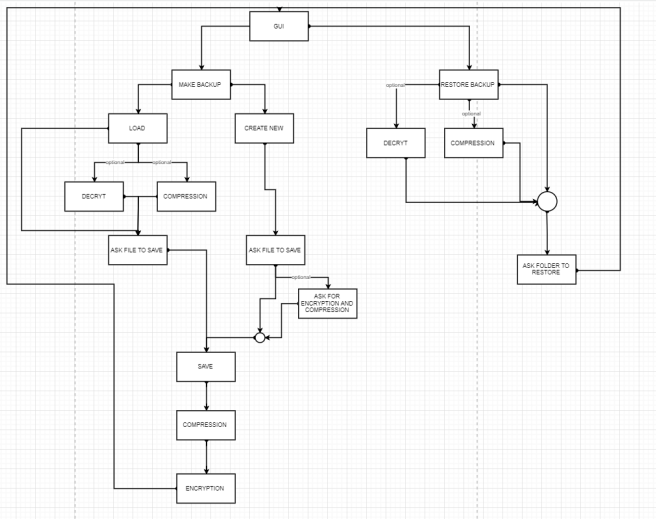
\includegraphics[width=13.1cm]{images/graph_gui.png}
		\caption{Graphe de l'interface}
		\label{Graphe de l'interface}
	\end{figure}
\newpage
	Le GUI est structuré de la manière suivante:\\ \\
	- GUI : La première fenêtre permet de choisir si l'utilisateur désire crée un nouveau un backup ou restaurer un backup.\\\\
	- Make Backup: Demande à l'utilisateur s'il veut créer un nouveau Backup ou s'il en existe un déjà existant qu'il veut écraser.\\\\
	- Load et Create New: Demande à l'utilisateur les chemins vers le fichier à sauvegardé et le chemin vers le lieu ou sera stocker la sauvegarde (+ l'ancienne sauvegarde si Load est choisi). L'utilisateur est aussi demander s'il veut chiffrer et/ou compresser sa sauvegarde.
	- Save: Fait la sauvegarde avec les chemins récupérés.\\\\
	- Compression: Si la compression fut choisit, propose à l'utilisateur de choisir une mode de compresssion: Huffman ou lz78. Huffman ne demande aucune information, lz78 va demander un chemin vers un dictionnaire à l'utilisateur.\\\\
	- Encryption: Si le chiffrement fut choisit, propore à l'utilisateur de choisir entre plusieurs mode de chiffrement: Rotn (demande à l'utilisateur un entier 'int')/ Vigenere et AES (demande à l'utilisateur une chaîne de caractère) / RSA et ELGAMAL(demande à l'utilisateur s'il veut créer un set de clé-> génère une clé publique et une clé privé dans le chemin demander/ ou s'il veut utiliser une clé publique -> doit donner le chemin vers la clé).\\\\
	- Restore Backup: Demande le chemin du fichier à restaurer, et si l'utilisateur à utilisé du chiffrement et/ou de la compression.\\\\
	- Decrypt et Decompression: Déchiffre et décompresse avec les modes précédemment renseignés par l'utilisateur avec leur argument correspondant. \\\\
	- Restore: Restaure le fichier original du backup, après le déchiffrement et/ou la décompression si nécessaire.\\\\

    Dans le cahier des charges et lors des précédentes soutenances, certains objectifs ont été fixé et certain on été respectés, tandis que d'autre n'ont pas put être accomplit.
\newpage
    Respect des objectifs imposés:\\\\
    - Interface graphique pas surchargée et simple d'utilisation, facile à prendre en main.\\
    - Donne accès a plusieurs modes de compression et de chiffrement différents, donnant le choix à l'utilisateur.\\
    - Permet de récupérer les informations entrée par l'utilisateur pour les utilisé.\\\\
    
    Problèmes Majeurs:\\\\
    - Interface non fonctionnelle en terme d'utilisation pour le système de backup et de restauration: Le GUI ne règle lance pas les fonctions nécessaires -> Ce problème est majoritairement dut à la gestion de fichier temporaire qui est difficile à gérer dans l'interface graphique qui est mal organisé dans son code.\\
    - Un memory leak assez conséquent du à des problèmes lié à GTK qui n'ont pas été identifié.\\\\
    
    Problème Mineurs:\\\\
    - Manque de détails décoratifs qui avait été prévu d'implanter (une jauge de durée pour l'exécution des programmes ou des informations indiquant le succès des programmes).\\
    - Manque d'un onglet "help" qui avait été prévu d'implanter pour expliqué les différents types de chiffrement et de compression à l'utilisateur, et leur fonctionnement exacte.\\
    
    \begin{figure}[!h]
		\centering
		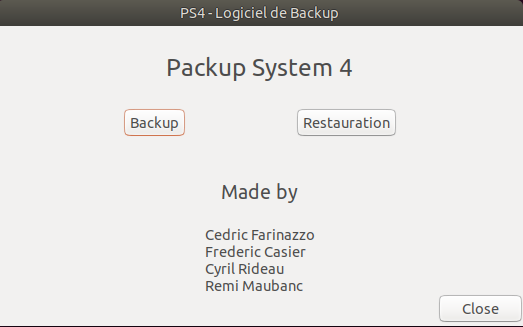
\includegraphics[width=10cm]{images/gui_screen.png}
		\caption{Interface graphique}
		\label{Interface graphique}
	\end{figure}

\newpage

\section{L'interface en ligne de commande (CLI)}
    Nous avons rajouté une interface en ligne de commande. Cette interface permet de faire exactement la même que l'interface graphique mais en ligne de commande. De cette façon, Packup peut être utilisé même sans serveur X.
    Cette interface est disponible grâce à l'argument "cli" de notre exécutable. \\
    
    Du à la différence d'implémentation, cette interface est totalement opération comparé à l'interface graphique.

    \begin{figure}[!h]
		\centering
		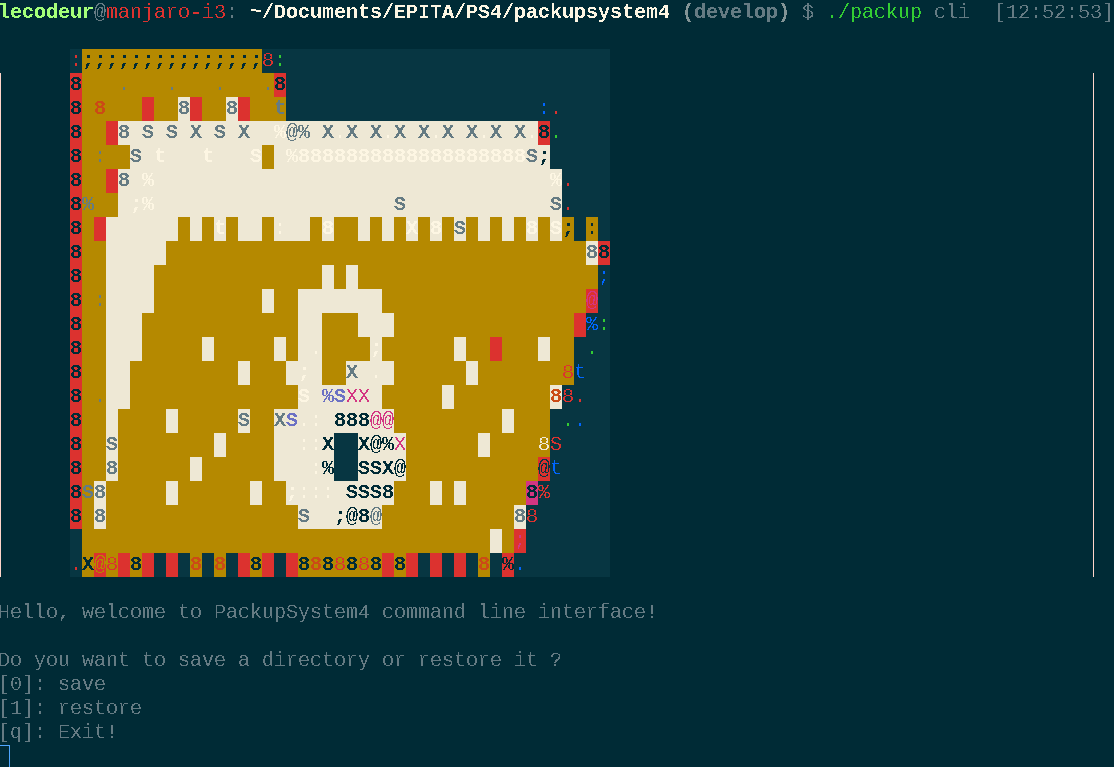
\includegraphics[width=15cm]{images/packup_cli.png}
		\caption{ Interface en ligne de commande }
		\label{ Interface en ligne de commande }
	\end{figure}
	
\newpage

\section{Site web}
    \begin{figure}[!h]
		\centering
		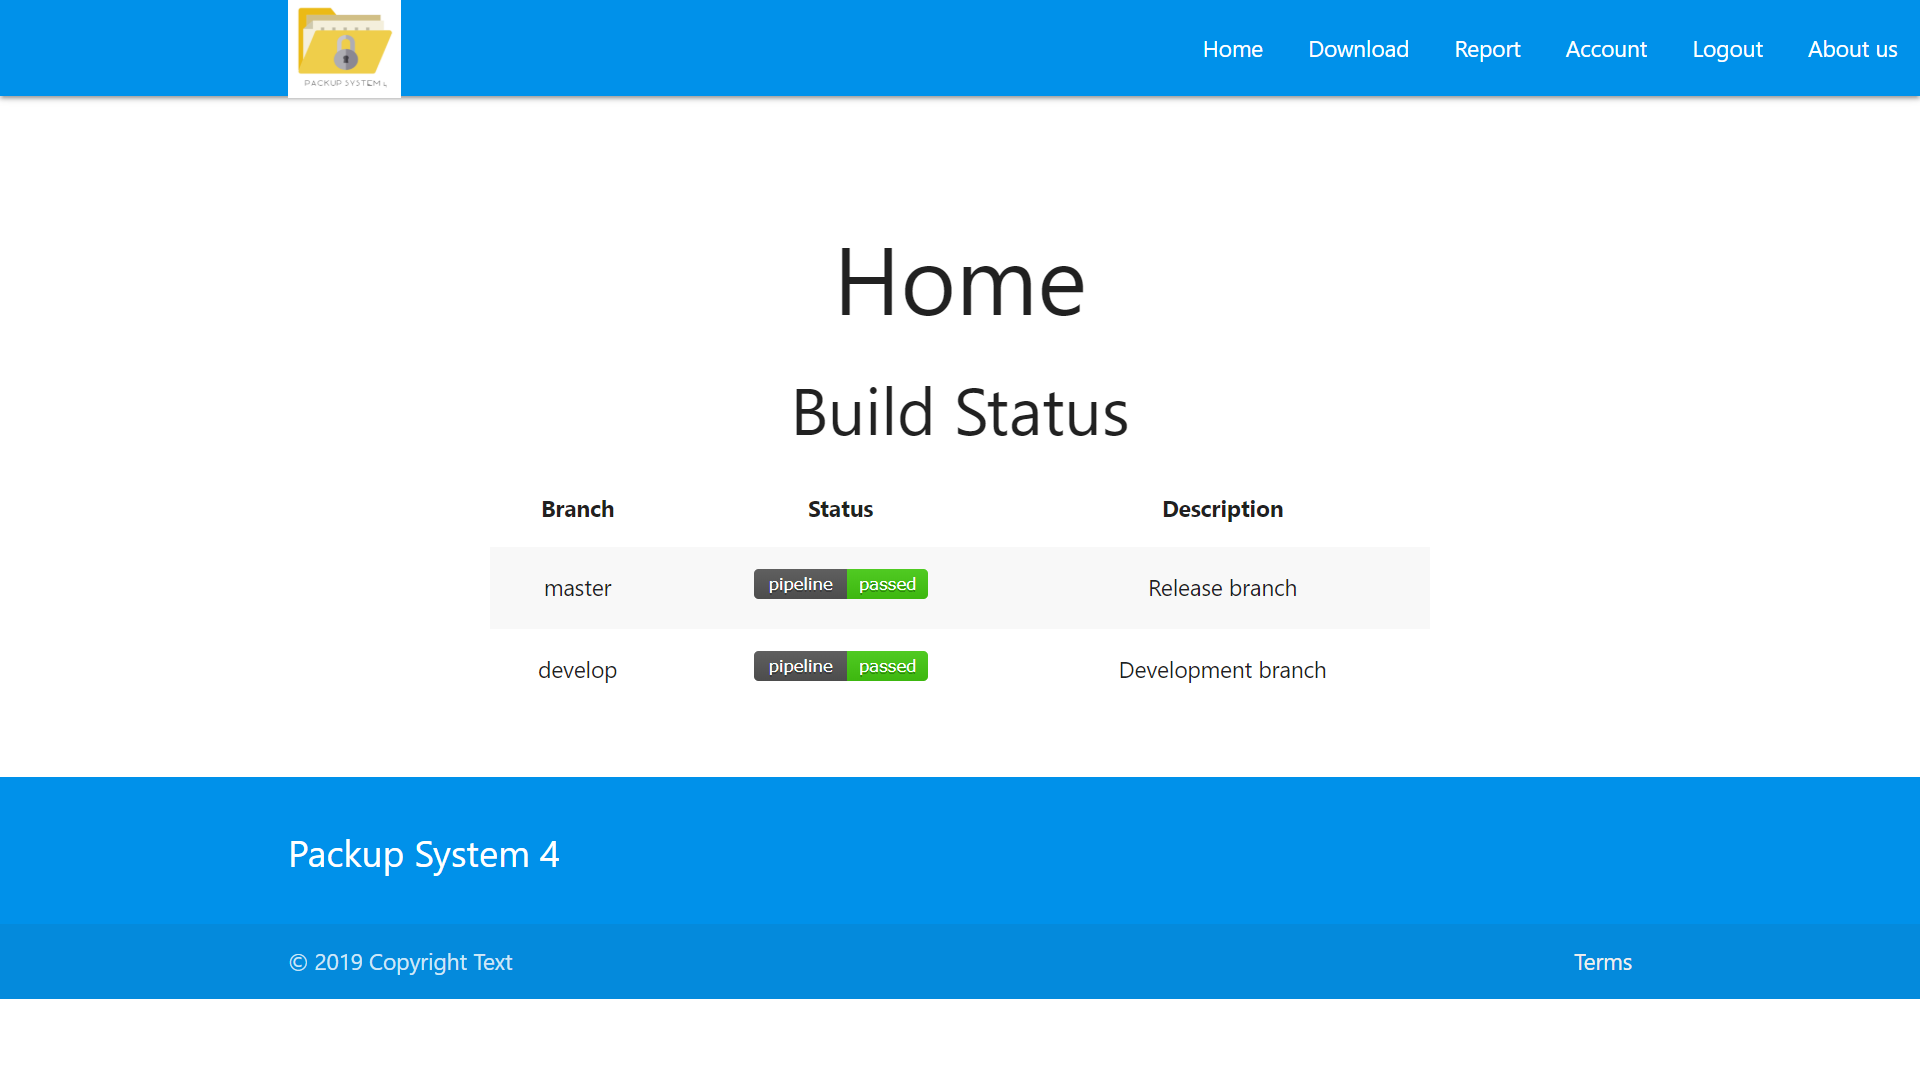
\includegraphics[width=8cm]{images/website.png}
		\caption{Site web actuel}
		\label{Site web actuel}
	\end{figure}
	\\
    Le site web est disponible à l'adresse suivante: \url{https://packup.hyperion.tf/}. \\
    Il est actuellement hébergé sur un VPS\footnote{VPS (Virtual Private Server) = Serveur privé virtuel} d'OVH déjà utilisé par Hyperion pour héberger plusieurs sites web. Ce serveur était idéal car il possède une configuration opérationnelle. Notre choix pour les parties de back-end et de front-end ont été très largement influencé par les infrastructure web déjà en place. Ainsi, nous avons choisit le framework Django \url{https://www.djangoproject.com/} pour le site web qui fait appel au serveur d'application uwsgi et au reverse proxy nginx.
    Pour le style et l'affichage, nous utilisons le framework Materialize (\url{https://materializecss.com/}) afin de vous présenter un site web clair et responsive.

    Notre cahier des charges et les rapports de soutenance sont aussi disponibles sur ce dernier dans la section "Report". Egalement dans la section "Download" vous pouvez trouver des version compilées de notre projet.
    
    Comme prévu, pour cette soutenance, nous avons ajouté le système d'authentification.
    L'utilisateur peut donc créer un compte, se connecter, modifier ces informations.
    
    Pour la dernière soutenance, nous permettrons à l'utilisateur d'envoyer une archive générer par notre programme sur le site web.
    \begin{figure}[!h]
		\centering
		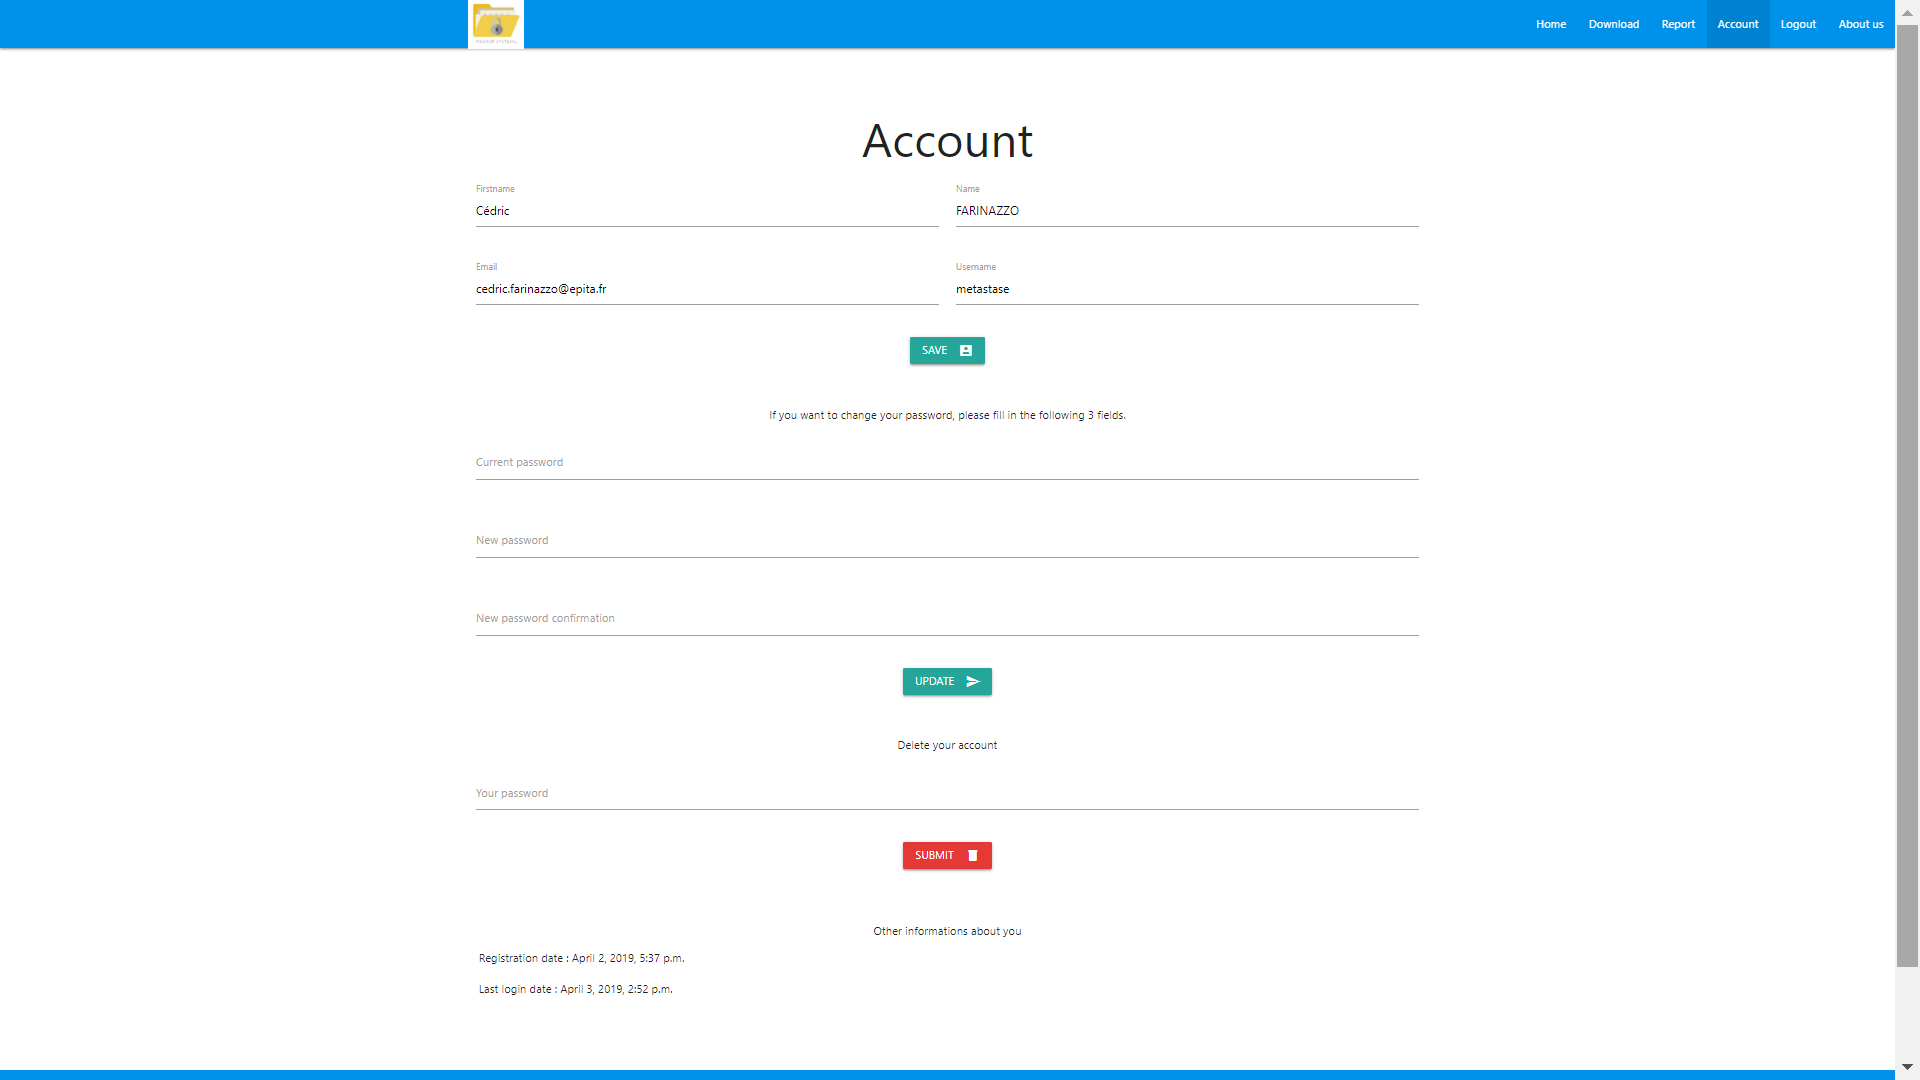
\includegraphics[width=8cm]{images/website-account.png}
		\caption{Page permettant de gérer les informations du compte}
		\label{Site web - Page permettant de gérer les informations du compte}
	\end{figure}
    
    \newpage

	Nous avons donc une interface de connexion qui donne accès à une interface permettant de télécharger ses backup. Arrivé sur cette interface, en haut à droite, nous pouvons avoir en temps réel le poids total actuel des backup situé sur le serveurs. Pour des raisons de sécurité le poids maximum par compte est de 5 Mo. De plus, si une requête d'upload dépasse les 6 Mo, le serveur nginx interrompra la requête en retournant une erreur 413 : Requête trop lourde. Au centre de la page nous pouvons voir les différentes backup déjà téléchargées (si elle existe) et leurs différents attributs (numéro d'identification dans le serveur, nom, type de compression, type de chiffrement, date de création) et un lien permettant de visualiser l'arbre des fichiers internes. 
	 \begin{figure}[!h]
		\centering
		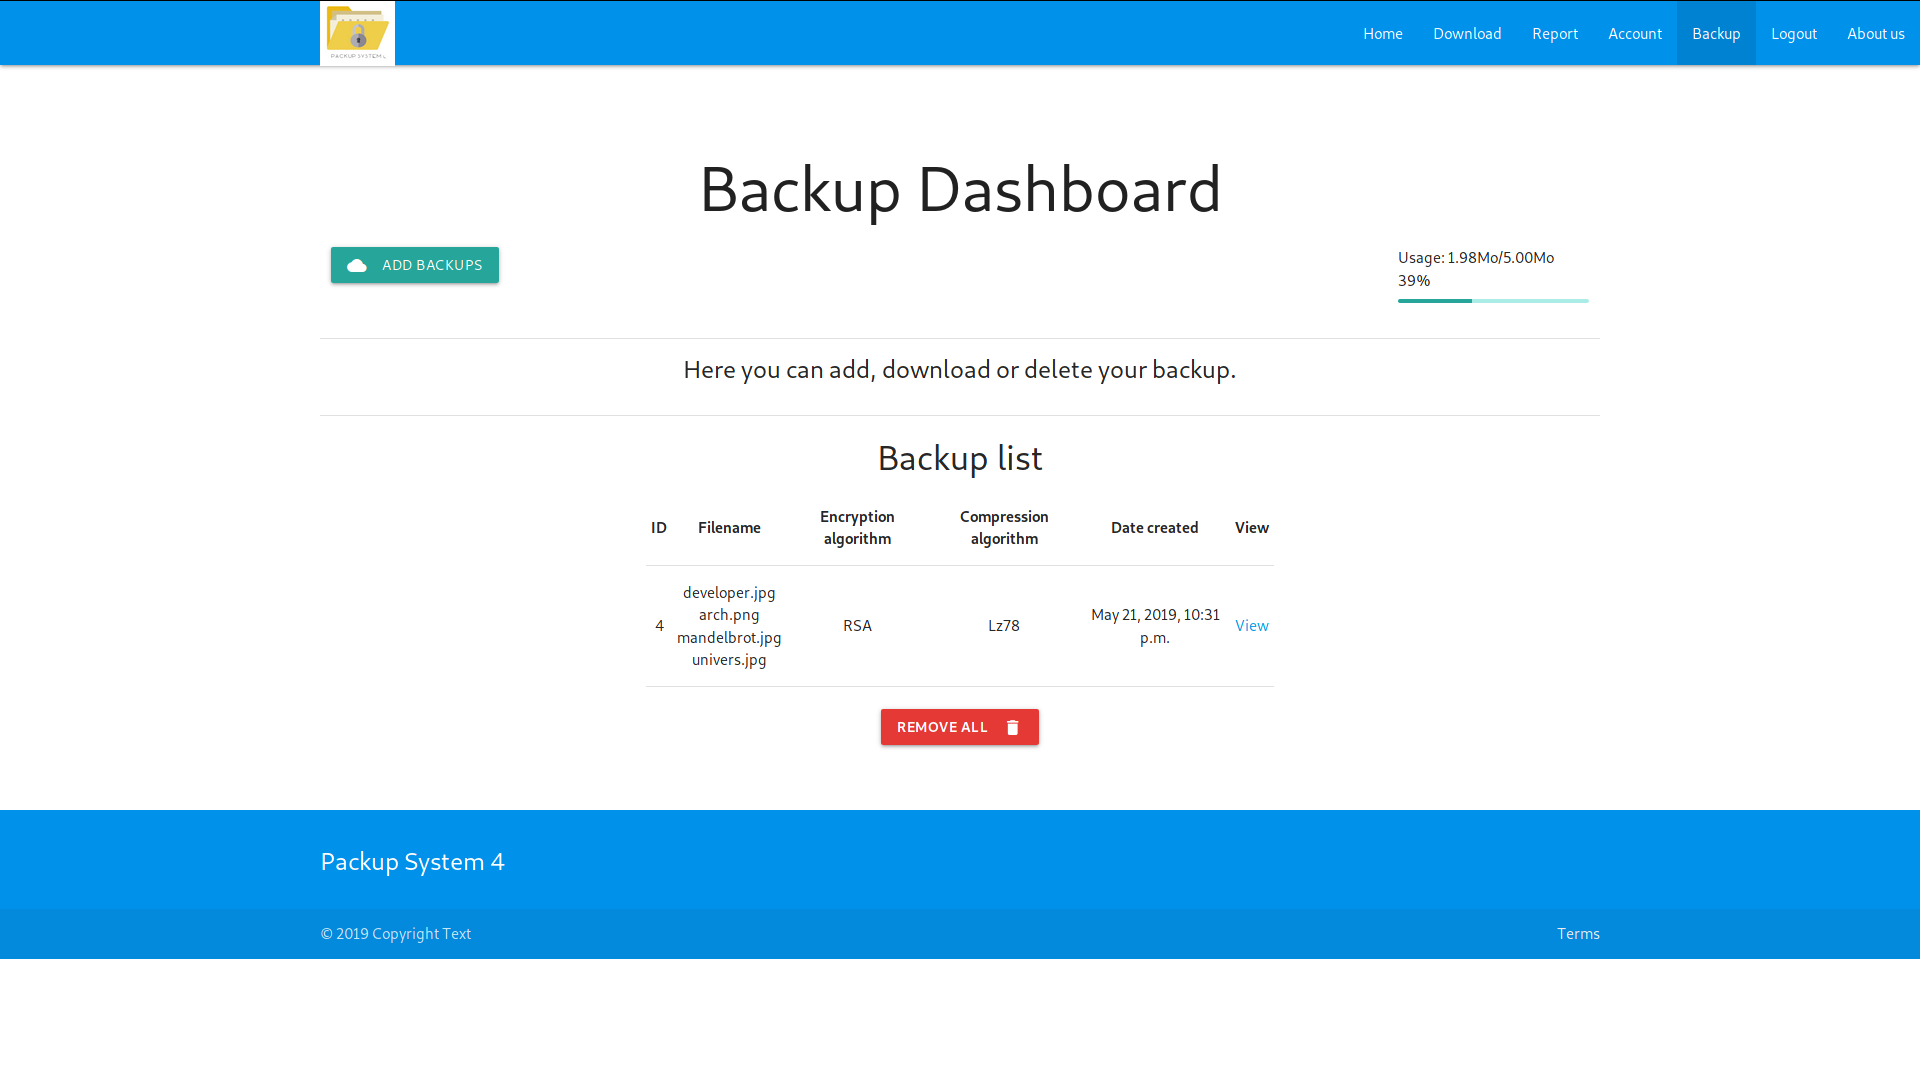
\includegraphics[width=8cm]{images/website_dashboard.png}
		\caption{Site web - Backup dashboard}
		\label{Site web - Backup dashboard}
	\end{figure}
	
	Nous avons également un bouton permettant de purger les backups chargées et un bouton redirigeant vers une page pour upload une nouvelle backup.\\
	Sur cette page on peut choisir le ou les fichiers choisir les algorithmes de compression et de chiffrement. En fonction des choix de l'utilisateur, des entrées supplémentaires s'ajoute comme pour upload le dictionnaire pour lz78 ou les clés pour rsa et elgamal. Ou encore la phrase clé pour aes ou vigenere. Pendant le submit, des erreurs peuvent survenir comme un dépassement sur l'espace disponible.
	\begin{figure}[!h]
		\centering
		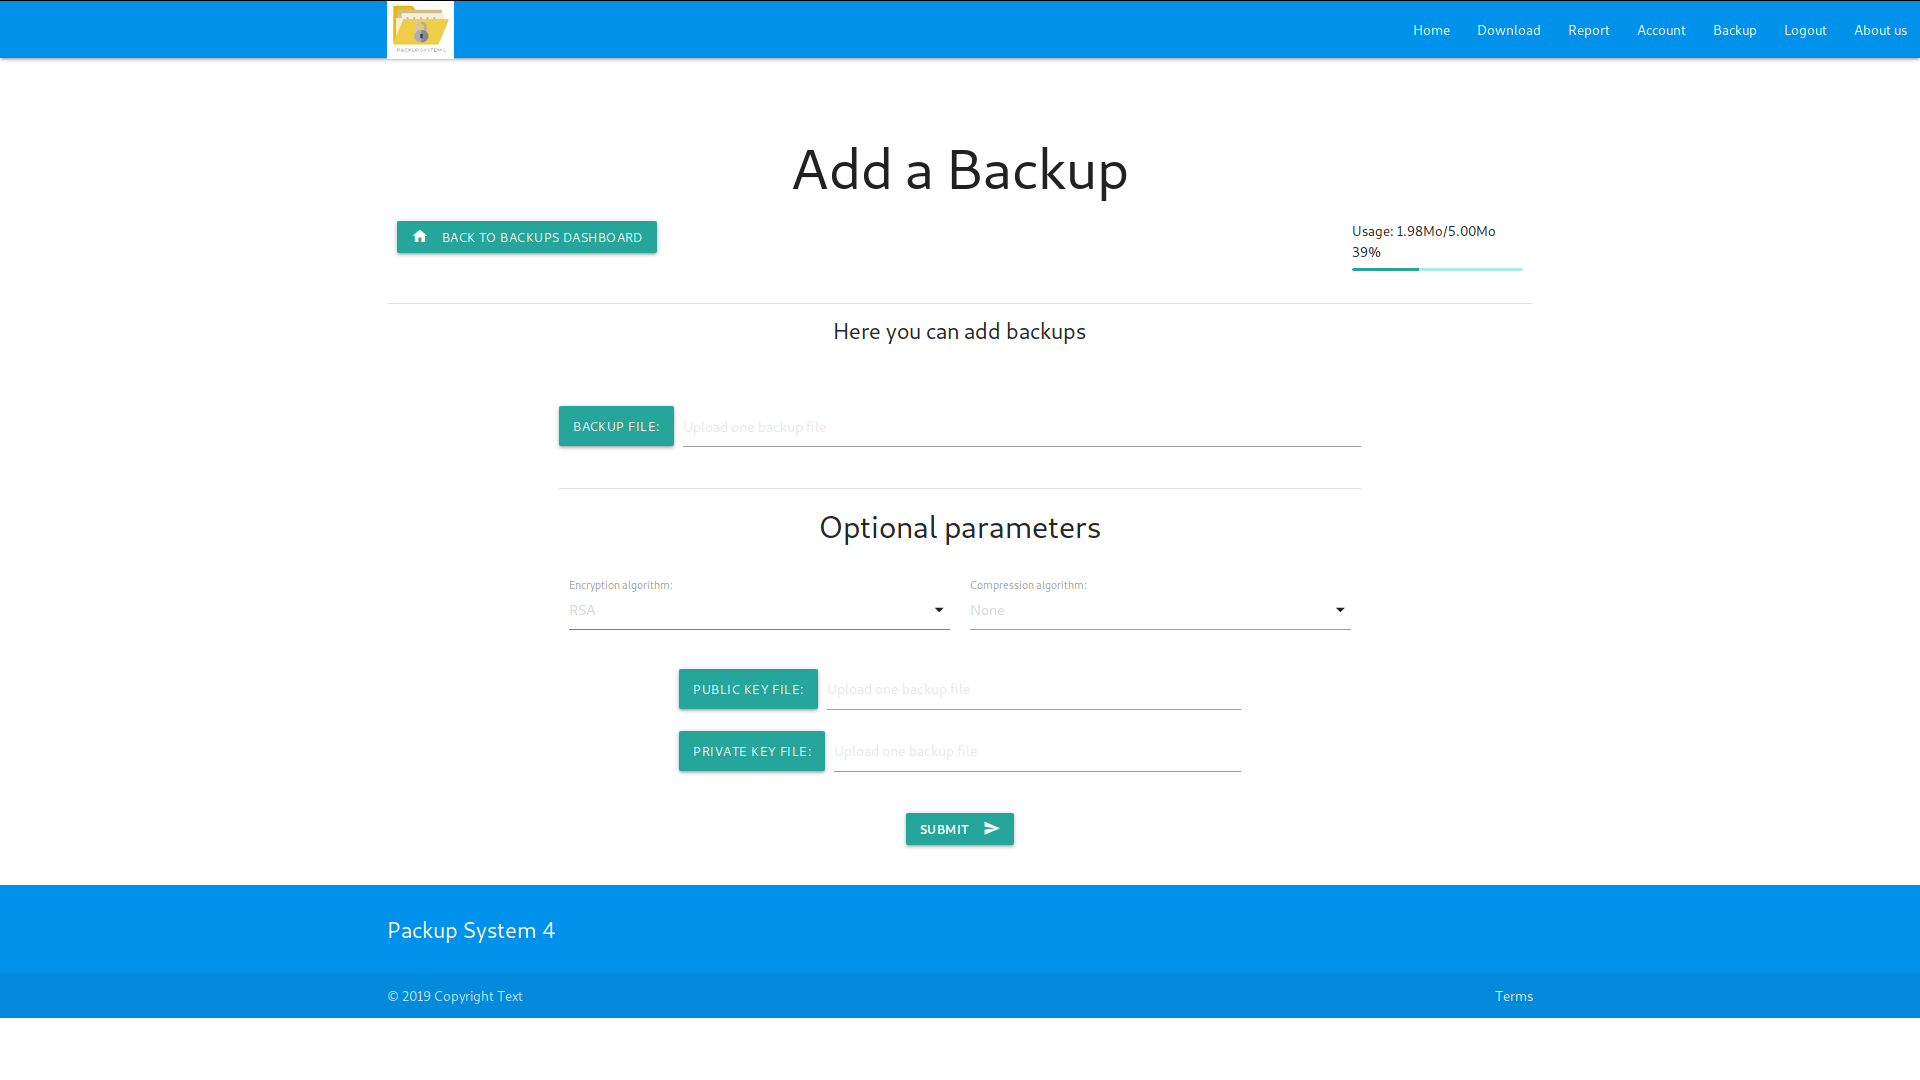
\includegraphics[width=8cm]{images/website_add_backup.png}
		\caption{Site web - Page d'ajout des backups}
		\label{Site web - Page d'ajout des backups}
    \end{figure}
	
	\newpage
	
	Sur la page de visualisation de l'archive on peut la liste des fichiers après déchiffrement et décompression grâce au programme s'exécutant sur le serveur. Cependant cette partie bonus n'a pas pu aboutir dans le temps imparti.
	\begin{figure}[!h]
		\centering
		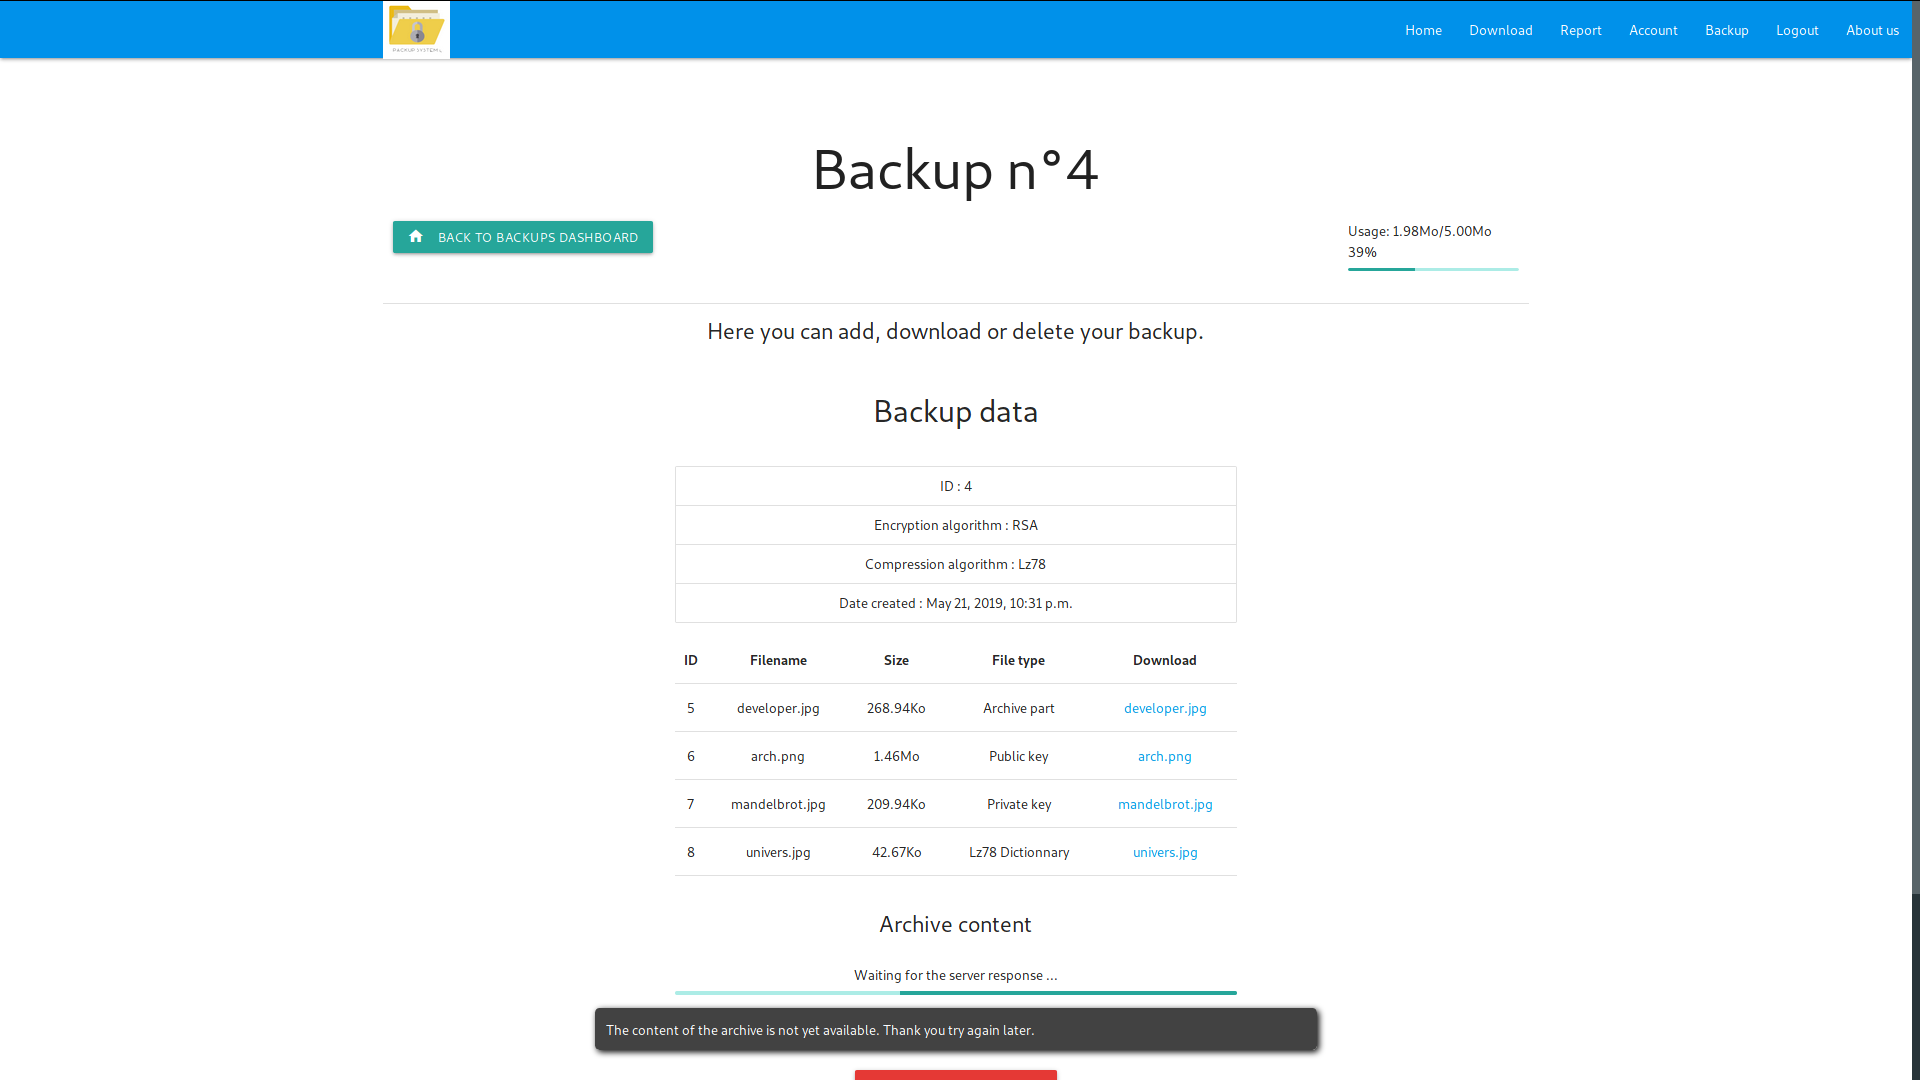
\includegraphics[width=8cm]{images/website_backup.png}
		\caption{Site web - Page de présentation des backup}
		\label{Site web - Page de présentation des backup}
	\end{figure}
	
\newpage
